\documentclass[semifinal]{cpecmu}

%% This is a sample document demonstrating how to use the CPECMU
%% project template. If you are having trouble, see "cpecmu.pdf" for
%% documentation.

\projectNo{P025-2}
\acadyear{2023}

\titleTH{การวิเคราะห์เชิงเปรียบเทียบของโมเดลทางภาษาสำหรับการจำแนกประเภท ESG}
\titleEN{Comparative Analysis of ESG-NLP classification model}

\author{นายสุภาค ไชยเนตรเกษม}{Supak Chainetkasem}{630610769}
\author{นายธนิสร ไชยวุฒิ}{Thanisorn Chaiwut}{630610738}

\cpeadvisor{patiwet}
\cpecommittee{natthanan}
\cpecommittee{karn}

%% Some possible packages to include:
\usepackage[final]{graphicx} % for including graphics

%% Add bookmarks and hyperlinks in the document.
\PassOptionsToPackage{hyphens}{url}
\usepackage[colorlinks=true,allcolors=Blue4,citecolor=red,linktoc=all]{hyperref}
\def\UrlLeft#1\UrlRight{$#1$}

%% Needed just by this example, but maybe not by most reports
\usepackage{afterpage} % for outputting
\usepackage{pdflscape} % for landscape figures and tables. 

%% Some other useful packages. Look these up to find out how to use
%% them.
% \usepackage{natbib}    % for author-year citation styles
% \usepackage{txfonts}
% \usepackage{appendix}  % for appendices on a per-chapter basis
% \usepackage{xtab}      % for tables that go over multiple pages
% \usepackage{subfigure} % for subfigures within a figure
% \usepackage{pstricks,pdftricks} % for access to special PostScript and PDF commands
% \usepackage{nomencl}   % if you have a list of abbreviations

%% if you're having problems with overfull boxes, you may need to increase
%% the tolerance to 9999
% \tolerance=9999

\bibliographystyle{plain}
% \bibliographystyle{IEEEbib}

% \renewcommand{\topfraction}{0.85}
% \renewcommand{\textfraction}{0.1}
% \renewcommand{\floatpagefraction}{0.75}

%% Example for glossary entry
%% Need to use glossary option
%% See glossaries package for complete documentation.
\ifglossary
  \newglossaryentry{lorem ipsum}{
    name=lorem ipsum,
    description={derived from Latin dolorem ipsum, translated as ``pain itself''}
  }
\fi

%% Uncomment this command to preview only specified LaTeX file(s)
%% imported with \include command below.
%% Any other file imported via \include but not specified here will not
%% be previewed.
%% Useful if your report is large, as you might not want to build
%% the entire file when editing a certain part of your report.
% \includeonly{chapters/intro,chapters/background}

\begin{document}
\maketitle
\makesignature

\ifproject
\begin{abstractTH}


ในปัจจุบันนักลงทุนได้ตระหนักว่าความพยายามในการทํากําไรเพื่อเอาชนะแนวโน้มของตลาดการลงทุนเป็นเรื่องที่ยาก 
นักลงทุนทั่วโลกจึงหันมาให้ความสนใจกับการลงทุนในบริษัทที่ให้ความสําคัญกับพัฒนาองค์กรอย่างยั่งยืน ซึ่งประกอบไปด้วยสามด้านหลักคือ 
ด้านสิ่งแวดล้อม(Environment), ด้านสังคม(Social) และด้านธรรมาภิบาล(Governance) 
โดยมีแนวคิดคือการลงทุนที่เน้นความยั่งยืนจะนํามาซึ่งผลตอบแทนที่มากขึ้นตามไปด้วย 
ในงานวิจัยนี้จะเน้นไปที่การเก็บรวบรวมรายงานผลประกอบการประจําปีจากบริษัทในดัชนีSETของตลาดหลักทรัพย์แห่งประเทศไทยนํามาแบ่งประโยคและจำแนกแต่ละประโยคเพื่อดูว่าแต่ละบริษัทมีประโยคที่เกี่ยวข้องกับด้านสิ่งแวดล้อม(Environment), 
ด้านสังคม(Social), ด้านธรรมาภิบาล(Governance)
หรือไม่เกี่ยวข้องกับด้านใดเลย(Neutral) มากเพียงใดด้วยโมเดลด้านภาษาธรรมชาติ และหาว่าโมเดลด้านภาษาธรรมชาติแบบใดที่สามารถจำแนกประโยคในรายงานประจำปีว่าเป็นด้านสิ่งแวดล้อม(Environment),
ด้านสังคม(Social) หรือด้านธรรมาภิบาล(Governance)หรือไม่เกี่ยวข้องกับด้านใดเลย(Neutral)ได้ดีที่สุด
\end{abstractTH}

\begin{abstract}


    Nowadays, investors have realized that it is difficult to make profitable attempts to overcome the trend of the investment market. 
    Investors around the world have therefore turned their attention to investing in companies that place importance on sustainable organizational development. 
    which consists of three main aspects: Environmental, Social, and Governance, with the idea that investments that emphasize sustainability will bring greater returns as well. 
    In this research, we will focus on collecting annual reports from companies in the SET Index of the Stock Exchange of Thailand. Divide it into sentences 
    and classify each sentence to see how many sentences in each company relate to the environment (Environment), society (Social), governance (Governance),
     or not related to any aspect at all(Neutral) with natural language models and find the best natural language model that can classify sentences in annual reports as 
     environmental, social, or governance, or not related to any aspect at all (Neutral).
\end{abstract}

\iffalse
\begin{dedication}
This document is dedicated to all Chiang Mai University students.

Dedication page is optional.
\end{dedication}
\fi % \iffalse

\begin{acknowledgments}

    \enskip \enskip \enskip โครงงานนี้ได้รับความกรุณาจาก ผศ.ดร.ปฏิเวธ วุฒิสารวัฒนา อาจารย์ที่ปรึกษาที่ได้สละเวลาให้ความช่วยเหลือทั้งให้คำแนะนำให้ความรู้และแนวคิดต่างๆรวมถึง 
    ผศ.ดร.กานต์ ปทานุคม และ ผศ.ดร.ณัฐนันท์ พรหมสุข ที่ให้คำปรึกษาจนทำให้โครงงานเล่มนี้เสร็จสมบูรณ์ไปได้


    ขอบคุณคนใน Biomedical Imaging Lab ภาควิชาวิศวกรรมคอมพิวเตอร์ คณะวิศวกรรมศาสตร์ 
    มหาวิทยาลัยเชียงใหม่ ที่ได้ให้คำปรึกษาการทำโครงงานและให้สนับสนุนทางด้านสื่อการศึกษาออนไลน์ขอขอบคุณเพื่อนๆที่ให้กำลังใจลอดการทำโครงงานที่ผ่านมา
    
    
    นอกจากนี้ผู้จัดทำขอขอบพระคุณบิดา มารดาที่ได้ให้ชีวิต เลี้ยงดูสั่งสอน และส่งเสียให้กระผมได้ศึกษาเล่าเรียนจนจบหลักสูตรปริญญาตรี
    หลักสูตรวิศวกรรมศาสตรบัณฑิต ซึ่งท่านได้ให้กำลังใจตลอดมาจนทำให้โครงงานนี้สำเร็จ 
    รวมทั้งขอขอบพระคุณอีกหลายๆท่านที่ไม่ได้เอ่ยนามมา ณ ที่นี้ ที่ได้ให้ความช่วยเหลือตลอดมา 
    หากหนังสือโครงงานเล่มนี้มีข้อผิดพลาดประการใด กระผมขอน้อมรับด้วยความยินดี
\acksign{2024}{3}{29}
\end{acknowledgments}%
\fi % \ifproject

\contentspage

\ifproject
\figurelistpage

\tablelistpage
\fi % \ifproject

% \abbrlist % this page is optional

% \symlist % this page is optional

% \preface % this section is optional


\pagestyle{empty}\cleardoublepage
\normalspacing \setcounter{page}{1} \pagenumbering{arabic} \pagestyle{cpecmu}

\chapter{\ifenglish Introduction\else บทนำ\fi}

\section{\ifenglish Project rationale\else ที่มาของโครงงาน\fi}

    \enskip \enskip \enskip ในปัจจุบันการลงทุนในหุ้นนั้นถือเป็นหนึ่งในการลงทุนที่ดีที่สุด เนื่องจากการลงทุนในหุ้นนั้นมีข้อดีมากมาย
    เช่น การมีสภาพคล่องและผลตอบแทนที่สูง ความสามารถในการสร้างกระแสเงินสดจากเงินปันผล
    นอกจากนั้นถ้าถือในระยะยาวพอจะทำให้โอกาสในการขาดทุนนั้นมีน้อยมาก
    แต่การลงทุนในหุ้นก็ไม่ได้เหมาะกับคนทุกคน
    เนื่องจากหุ้นนั้นเป็นสินทรัพย์ที่มีความผันผวนของราคาสูง
    ดังนั้นคนที่รับความเสี่ยงได้น้อยก็จะไม่เหมาะกับการลงทุนประเภทนี้


    การลงทุนในหุ้นนั้นมีแนวทางมากมาย เช่น การลงทุนในหุ้นเติบโต 
    การลงทุนในหุ้นคุณค่าหรือการลงทุนโดยเน้นลงทุนในหุ้นที่ให้เงินปันผลที่สูง 
    โดยในโครงงานนี้จะนำเสนอแนวทางการลงทุนที่มีชื่อว่า 
    การลงทุนอย่างยั่งยืน (Sustainable Investment) โดยการลงทุนอย่างยั่งยืนนี้
    จะมุ่งเน้นการลงทุนไปยังบริษัทที่ให้ความสำคัญกับสามด้าน คือ สิ่งแวดล้อม (Environment), สังคม(Social)
    และธรรมาภิบาล (Governance) โดยจะมีการให้คะแนนทางด้านความยั่งยืนที่มีชื่อว่าคะแนน ESG

    โครงงานฉบับนี้มีจุดประสงค์สองอย่าง คือ สร้างระบบที่สามารถบ่งบอกได้ว่าบริษัทแต่ละบริษัทมีประโยคที่พูดถึงเกี่ยวกับประเด็นที่เกี่ยวข้องกับ ESG
    อยู่มากน้อยเพียงใดจากการให้ระบบอ่านรายงานประจำปีของบริษัทต่างๆ และพัฒนาโมเดลด้านภาษาธรรมชาติที่ดีที่สุดจากโมเดลด้านภาษาธรรมชาติหลายๆโมเดล
    เพื่อจำแนกว่าประโยคแต่ละประโยคในรางงานประจำปีพูดถึงหัวข้อใดใน ESG หรือไม่พูดถึงหัวข้อใดเลย
\section{\ifenglish Objectives\else วัตถุประสงค์ของโครงงาน\fi}
\begin{enumerate} 
    \item
    พัฒนาโปรแกรมเพื่อวิเคราะห์ประโยคว่าประโยคที่ปรากฏในรายงานประจำปีเป็นชนิด
    สิ่งแวดล้อม(Environment), สังคม (Social), ธรรมาภิบาล (Governance) 
    หรือประโยคที่ไม่เข้าชนิดใดเลย (Neutral) 
    โดยใช้โมเดลด้านภาษาธรรมชาติและค้นหาว่าโมเดลด้านภาษาธรรมชาติชนิดใดที่นำมาใช้กับงานนี้ได้ดีที่สุด
    \item
    พัฒนาโปรแกรมเพื่อวิเคราะห์รายงานประจำปีเพื่อหาว่ารายงานประจำปีที่วิเคราะห์มีประโยคชนิดสิ่งแวดล้อม(Environment),
    สังคม (Social), ธรรมาภิบาล (Governance) 
    และประโยคที่ไม่เข้าชนิดใดเลย (Neutral) อยู่มากน้อยเพียงใดโดยใช้โปรแกรมวิเคราะห์วิเคราะห์ประโยคที่พัฒนาจากโมเดลด้านภาษาธรรมชาติ
\end{enumerate}

\section{\ifenglish Project scope\else ขอบเขตของโครงงาน\fi}

\begin{enumerate} 
    \item
    ใช้ข้อมูลจากรายงานประจำปีที่เผยแพร่ในเว็บไซต์ของตลาดหลักทรัพย์แห่งประเทศไทยเท่านั้น
    \item
    ใช้รายงานประจำปีฉบับภาษาอังกฤษเท่านั้น
\end{enumerate}

% \subsection{\ifenglish Hardware scope\else ขอบเขตด้านฮาร์ดแวร์\fi}

% \subsection{\ifenglish Software scope\else ขอบเขตด้านซอฟต์แวร์\fi}

\section{\ifenglish Expected outcomes\else ประโยชน์ที่ได้รับ\fi}

    \enskip \enskip \enskip เนื่องจากข้อมูลเกี่ยวการพูดถึงประเด็นที่เกี่ยวข้องกับESGของบริษัทต่างๆมีการเปิดเผยข้อมูลที่น้อยมาก
    โดยถ้าอยากได้ข้อมูลที่มากขึ้นก็จะมีค่าใช้จ่ายเพิ่มเติมในการเปิดเผยข้อมูล 
    ทางผู้จัดทำจึงพัฒนาโปรแกรมขึ้นมาเพื่ออ่านรายงานประจำปีของบริษัทเพื่อดูว่าบริษัทนั้นมีการพูดถึงเกี่ยวกับประเด็นESGมากน้อยเพียงใด
    เพื่อที่จะไม่ต้องใช้แรงงานมนุษย์ในการหาข้อมูลจากรายงานประจำปี
    ดังนั้นจึงทำให้ต้นทุนในส่วนนี้หายไป 
    ข้อมูลนี้จึงสามารถเปิดเผยข้อมูลทั้งหมดได้โดยไม่มีค่าใช้จ่ายใด ๆ

\section{\ifenglish Technology and tools\else เทคโนโลยีและเครื่องมือที่ใช้\fi}

\subsection{\ifenglish Hardware technology\else เทคโนโลยีด้านฮาร์ดแวร์\fi}

\enskip \enskip \enskip Notebook Acer Nitro 7 AN715-51 และ Notebook Acer Nitro 5 AN515-51 สำหรับงานทั้งหมดในโครงงานนี้

\subsection{\ifenglish Software technology\else เทคโนโลยีด้านซอฟต์แวร์\fi}

\enskip \enskip \enskip ใช้Pythonในการเขียนโปรแกรมและใช้libraryดังนี้ Pandas ,NumPy ,Scikit Learn ,Tensorflow ,Keras ,Transformers ,Spacy ,PyTorch ,PyMuPDF ,Nltk

\section{\ifenglish Project plan\else แผนการดำเนินงาน\fi}

\begin{plan}{10}{2023}{3}{2024}
    \planitem{10}{2023}{10}{2023}{ศึกษาค้นคว้าข้อมูล}
    \planitem{11}{2023}{1}{2024}{เตรียมข้อมูลสำหรับพัฒนาโมเดลทางด้านภาษา}
    \planitem{12}{2023}{2}{2024}{พัฒนาโปรแกรมจำแนกประโยคและทดลองหาโมเดลทางด้านภาษาที่ดีที่สุด}
    \planitem{3}{2024}{3}{2024}{พัฒนาโปรแกรมอ่านรายงานประจำปีของบริษัท}
\end{plan}

\section{\ifenglish Roles and responsibilities\else บทบาทและความรับผิดชอบ\fi}
\enskip \enskip \enskip ผู้จัดทำทั้งสองคนช่วยกันทำงานทั้งหมดทุกส่วน แต่จะแบ่งงานหลักๆที่แต่ละคนได้ทำเป็นส่วนใหญ่ได้ดังนี้
นายสุภาค ไชยเนตรเกษม: รับผิดชอบหน้าที่ในการใช้การประมวลผลภาษาธรรมชาติเพื่อพัฒนาโปรแกรมจำแนกประโยคและทดลองเพื่อหาโมเดลทางด้านภาษาที่ดีที่สุด และเตรียมข้อมูลสำหรับพัฒนาโมเดลทางด้านภาษา
นายธนิสร ไชยวุฒิ: รับผิดชอบหน้าที่ในการเตรียมข้อมูลสำหรับพัฒนาโมเดลทางด้านภาษา ศึกษาหาข้อมูลอ้างอิงที่จะนำมาใช้ในงานส่วนต่างๆ และพัฒนาโปรแกรมอ่านรายงานประจำปีของบริษัท

\section{\ifenglish%
Impacts of this project on society, health, safety, legal, and cultural issues
\else%
ผลกระทบด้านสังคม สุขภาพ ความปลอดภัย กฎหมาย และวัฒนธรรม
\fi}

\enskip \enskip \enskip ผลกระทบทางด้านสังคม: ระบบที่เป็นผลลัพธ์ของโครงงานนี้จะสามารถใช้เพื่อเป็นตัวช่วยสำหรับนักลงทุนทั่วไปที่สนใจในการลงทุนเชิงยั่งยืน 
เนื่องจากในปัจจุบันนี้ข้อมูลเกี่ยวกับผลการดำเนินงานทางด้าน ESG ของบริษัทยังมีไม่มากนัก 
จึงหวังว่าระบบที่ถูกพัฒนามานี้จะสามารถช่วยได้ไม่มากก็น้อย


ผลกระทบทางด้านสุขภาพ: ตัวระบบที่ถูกพัฒนาขึ้นมานั้นไม่ส่งผลกระทบต่อสุขภาพแต่อย่างใด


ผลกระทบทางด้านกฎหมาย: ข้อมูลที่ใช้ในโครงงานนี้รวมไปถึงซอฟต์แวร์ที่ใช้ในการพัฒนานั้นทั้งหมดล้วนเป็นสิ่งที่สามารถหาได้ทั่วไปโดยไม่ละเมิดลิขสิทธิ์ 
ดังนั้นการทำโครงงานนี้จึงไม่มีผลกระทบด้านกฎหมายอย่างแน่นอน


ผลกระทบทางด้านวัฒนธรรม: ตัวระบบที่ถูกพัฒนาขึ้นมานั้นไม่มีผลกระทบทางด้านวัฒนธรรมแต่อย่างใด

\chapter{\ifenglish Background Knowledge and Theory\else ทฤษฎีที่เกี่ยวข้อง\fi}

การทำโครงงาน เริ่มต้นด้วยการศึกษาค้นคว้า ทฤษฎีที่เกี่ยวข้อง หรือ งานวิจัย/โครงงาน ที่เคยมีผู้นำเสนอไว้แล้ว ซึ่งเนื้อหาในบทนี้ก็จะเกี่ยวกับการอธิบายถึงสิ่งที่เกี่ยวข้องกับโครงงาน เพื่อให้ผู้อ่านเข้าใจเนื้อหาในบทถัดๆ ไปได้ง่ายขึ้น

\section{Data Cleaning}


\enskip \enskip \enskip กระบวนการตรวจสอบ สะสาง แก้ไข หรือจัดรูปแบบข้อมูลให้อยู่ในสภาพที่พร้อมใช้งานที่สุด
รวมไปถึงคัดกรองข้อมูลที่ไม่ถูกต้องหรือไม่จำเป็นออกไปจากชุดข้อมูลที่จะใช้วิเคราะห์หรือประมวลผล 
เพื่อให้ชุดข้อมูลที่จะใช้มีความสมบูรณ์ มีคุณภาพ พร้อมนำไปวิเคราะห์และใช้ประโยชน์


\section{Bidirectional Encoder Representations from Transformers (BERT)}
\enskip \enskip \enskip Bert มีชื่อเต็มว่า Bidirectional Encoder Representations from Transformersคือ 
โมเดลที่ต่อยอดมาจากโมเดลที่เรียกว่า Transformers ซึ่งถูกออกแบบมาให้เลือกใช้เฉพาะส่วนที่เป็น 
encoder ทำหน้าที่ในการแปลงคำในประโยคให้กลายเป็นเวกเตอร์ 
จากนั้นจึงใช้วิธีการฝึกโมเดลในรูปแบบที่ต่างออกไปจากโมเดลทางภาษาอื่นๆ ซึ่งการฝึกของ BERT จะแบ่งออกเป็นสองส่วนได้แก่

\subsection{Masked Language Model}

\enskip \enskip \enskip เป็นการฝึกโมเดลโดยคำในประโยคที่ป้อนเข้ามาเป็นอินพุตของระบบจะถูกลบออกไปบางส่วนและเรียกคำที่ถูกลบออกไปนี้ว่า 
(Masked words) โมเดลจะต้องพยายามเติมคำที่หายไปเหล่านี้ให้ถูกต้องซึ่งหากโมเดลจะสามารถเติมคำได้ถูกต้อง
การเรียนรู้แบบนี้ช่วยให้โมเดลสามารถเรียนรู้ความสัมพันธ์และบริบทของคำในประโยคได้ดีโดยข้อมูลที่นำมาใช้ในการฝึกโมเดลเป็นคลังข้อมูลทางภาษาที่มีขนาดใหญ่ 
เช่น Wikipedia

\subsection{Fine Tuning on Specific Tasks}

\enskip \enskip \enskip เป็นการเพิ่ม Layer พิเศษเข้าไปในชั้นเอาท์พุตของโมเดล 
โดย Layer พิเศษเหล่านี้จะสามารถทำให้โมเดลมีความสามารถอื่นเพิ่มเติม 
เช่น สามารถประมวลผลได้ว่าประโยคที่รับเข้ามามีใจความที่เป็นแง่บวกหรือแง่ลบ,
ความสามารถในการตอบคำถาม รวมถึงความสามารถในการแปลภาษา
จากข้อมูลข้างต้น ด้วยความสามารถที่มากกว่าโมเดลทางภาษาแบบอื่นและความสะดวกสบายในการปรับใช้งานได้หลากหลายรูปแบบ 
ทำให้โมเดลทางภาษาแบบ BERT เป็นโมเดลทางภาษาที่ได้รับความนิยมเป็นอย่างมากและถูกใช้งานในหลายภาคส่วน 
เช่น ระดับอุตสาหกรรมและในเชิงวิชาการ

% \subsubsection{Subsubsection 1 heading goes here}
% Subsubsection 1 text

% \subsubsection{Subsubsection 2 heading goes here}
% Subsubsection 2 text

\section{Recurrent Neural Network (RNN)}
\enskip \enskip \enskip เแบบหนึ่งที่ออกแบบมาแก้ปัญหาสำหรับงานที่ข้อมูลมีลำดับ
Sequence โดยใช้หลักการ Feed สถานะภายในของโมเดลกลับมาเป็น Input ใหม่ คู่กับ Inputปกติ เรียกว่า
Hidden State, Internal State, Memory ช่วยให้โมเดลรู้จำ Pattern ของลำดับ
Input Sequence ได้

\subsection{Long-Short Term Memory (LSTM)}

\enskip \enskip \enskip จากปัญหาที่เกิดขึ้นใน RNNs เกี่ยวกับค่า gradient ที่มีค่าน้อยลงจากการทำงานของ backpropagation
จึงได้มีการคิดค้น machine learning ตัวใหม่ที่ใช้หลักการคล้าย ๆ เดิม แต่เปลี่ยนตัวฟังก์ชันด้านในให้มีความเสถียรและมีประสิทธิภาพมากขึ้น 
ซึ่งนั่นก็คือ Long Short-Term Memoryหรือเรียกย่อๆว่า LSTMs สิ่งที่โดดเด่นขึ้นมานั้นก็คือการที่มันสามารถเลือกได้ว่าข้อมูลไหนที่ควรจะจดจำ
ข้อมูลไหนที่ควรจะกำจัดทิ้งออกไปผ่านการลืมของสถานะใน node นั้น ๆ

\section{ELECTRA}

\enskip \enskip \enskip โมเดล ELECTRA เป็นโมเดลทางภาษาที่นำเสนอเป็นวิธีการ pretraining ใหม่ๆ โดยการฝึกโมเดล transformer สองตัว คือ generator และ discriminator 
โดยที generator มีบทบาทในการแทนที่โทเค็นในลำดับและจึงถูกฝึกเป็น masked language model ในขณะที่ discriminator 
ซึ่งเป็นโมเดลที่เราสนใจพยายามระบุว่าโทเค็นไหนถูกแทนที่โดย generator ในลำดับนั้นๆ
% \begin{center}
% \begin{minipage}{2em}
% juxtaposition
% \end{minipage}
% \end{center}

\section{การลงทุนอย่างยั่งยืน}

\enskip \enskip \enskip หมายถึง แนวคิดการลงทุนที่คำนึงถึงการดำเนินงานด้านสิ่งแวดล้อม 
สังคม และบรรษัทภิบาลของธุรกิจประกอบการพิจารณาตัดสินใจลงทุนควบคู่ไปกับการวิเคราะห์ข้อมูลทางการเงินของธุรกิจ 
เพื่อสร้างผลตอบแทนในระยะยาวและสร้างผลกระทบเชิงบวกหรือลดผลกระทบเชิงลบต่อสังคมและสิ่งแวดล้อม

\section{\ifenglish%
\ifcpe CPE \else ISNE \fi knowledge used, applied, or integrated in this project
\else%
ความรู้ตามหลักสูตรซึ่งถูกนำมาใช้หรือบูรณาการในโครงงาน
\fi
}

\enskip \enskip \enskip จากหลักสูตรที่ได้เรียนทั้งหมดที่ผ่านมาทำให้ได้ความรู้จากวิชา 261448 หรือ Data Mining For CPE ที่มีความรู้พื้นฐานเกี่ยวกับการเรียนรู้ของเครื่อง และวิชา
261456 หรือ Intro Computer Intelligence For CPE ที่มีความรู้เกี่ยวกับโครงข่ายประสาทเทียมและวิชา
261459 หรือ Deep Learning ที่่มีความรู้เกี่ยวกับพื้นฐานเกี่ยวกับการเรียนรู้เชิงลึกและวิชา
261499 หรือ Natural Language Processing ที่่มีความรู้เกี่ยวกับพื้นฐานเกี่ยวกับการประมวลผลภาษาธรรมชาติ นำมาใช้เป็นแนวคิดในการพัฒนาตัวโครงงานนี้


\section{\ifenglish%
Extracurricular knowledge used, applied, or integrated in this project
\else%
ความรู้นอกหลักสูตรซึ่งถูกนำมาใช้หรือบูรณาการในโครงงาน
\fi
}

\enskip \enskip \enskip ความรู้ในทางการเงินในการอ่านรายงานประจำปีและวิธีจำแนกประโยคว่าประโยคนั้นๆมีหัวข้อใดบ้างใน ESG เพื่อหาข้อมูลมาใช้ในการพัฒนาโมเดล

\chapter{\ifproject%
\ifenglish Project Structure and Methodology\else โครงสร้างและขั้นตอนการทำงาน\fi
\else%
\ifenglish Project Structure\else โครงสร้างของโครงงาน\fi
\fi
}

\makeatletter

% \renewcommand\section{\@startsection {section}{1}{\z@}%
%                                    {13.5ex \@plus -1ex \@minus -.2ex}%
%                                    {2.3ex \@plus.2ex}%
%                                    {\normalfont\large\bfseries}}

\makeatother
%\vspace{2ex}
% \titleformat{\section}{\normalfont\bfseries}{\thesection}{1em}{}
% \titlespacing*{\section}{0pt}{10ex}{0pt}

\section{การเตรียมข้อมูล}

% \begin{figure}
% \begin{center}
% \includegraphics{800px-Briny_Beach.jpg}
% \end{center}
% \caption[Poem]{The Walrus and the Carpenter}
% \label{fig:walrus}
% \end{figure}

\subsection{ดาวน์โหลดข้อมูล}

\enskip \enskip \enskip เก็บเอกสารรายงานประจำปีย้อนหลังไม่เกิน 5 ปี จากเว็ปไซต์ของตลาดหลักทรัพย์แห่งประเทศไทย
โดยเอกสารจะอยู่ในรูปแบบไฟล์ PDF เพื่อเตรียมสำหรับจัดทำข้อมูลประโยคที่เกี่ยวข้องกับการดำเนินงาน
ที่ให้ความสำคัญกับ สิ่งแวดล้อม(Environment), สังคม(Social) และธรรมาภิบาล(Governance) 

\subsection{แบ่งรายงานประจำปีเป็นประโยค}

\enskip \enskip \enskip สร้างโปรแกรมแบ่งประโยคที่เมื่อนำรายงายประจำปีเข้าไปแล้วโปรแกรมจะตัดประโยคที่ไม่สมบูรณ์หรือพวกของที่ไม่จำเป็น 
เช่น ตาราง และหัวข้อ ออกไปและคัดมาให้แค่ประโยคที่สามารถใช้กับโมเดลได้ออกมาเป็นผลลัพธ์


\subsection{เลือกข้อมูลที่จะนำไปใช้พัฒนาโปรแกรม}

\enskip \enskip \enskip สุ่มอ่านประโยคในรายงานประจำปีของบริษัทที่เป็นผลลัพธ์ของโปรแกรมแบ่งประโยคที่เตรียมเอาไว้เพื่อเตรียมข้อมูลประโยคประเภทสิ่งแวดล้อม(Environment), 
สังคม(Social), ธรรมาภิบาล(Governance) และประโยคที่ไม่เข้าประเภทใดเลย(Neutral) โดยใชเกณฑ์จากคู่มือของตลาดหลักทรัพย์แห่งประเทศไทย ~\cite{sus}
  

\subsection{การทำความสะอาดข้อมูล}

\enskip \enskip \enskip นำประโยคที่เลือกมาทำการทำความสะอาดข้อมูลก่อนนำไปใช้กับโมเดล 
โดยวิธีการที่ใช้ทำความสะอาดข้อมูลคือ การตัดเครื่องหมายหรือสัญลักษณ์พิเศษต่างๆออก, การตัดurlออก, การเปลี่ยนตัวอักษรทั้งหมดเป็นตัวพิมเล็ก และการลบคำหยุดออก


\section{การพัฒนาโมเดลการเรียนรู้ของเครื่อง}

\enskip \enskip \enskip พัฒนาโมเดลการเรียนรู้ของเครื่องเพื่อนำมาทำนายชนิดของประโยคว่าเป็นหัวข้อใดในESGหรือไม่เกี่ยวข้องกับหัวข้อใดเลย 
โดยทดลองกับโมเดลหลายแบบซึ่งโมเดลที่เลือกได้แรงบันดาลใจมาจากงานวิจัย BERT goes sustainable : an NLP approach to ESG financing~\cite{torroni2021bert} ได้แก่โมเดล Bert~\cite{devlin2018bert}, Distilbert~\cite{sanh2019distilbert}, Albert-V2~\cite{lan2019albert}, Electar-base~\cite{clark2020electra}, Electar-small~\cite{clark2020electra}, Roberta~\cite{liu2019roberta}และใช้ LSTM~\cite{staudemeyer2019understanding} เป็นโมเดลพื้นฐานการวัดผลแล้วเลือกโมเดลที่ดีที่สุดโดยวัดประสิทธิภาพจากค่า Accuracy


\section{การพัฒนาโปรแกรมอ่านรายงานประจำปีของบริษัท}

\enskip \enskip \enskip นำโมเดลการเรียนรู้ของเครื่องที่ดีที่สุดที่พัฒนามาได้มาสร้างโปรแกรมนับจำนวนประโยคแต่ละชนิดในรายงานประจำปีที่ใส่เข้าไปเป็นอินพุต
เพื่อดูว่ารายงานประจำปีที่ใส่เข้าไปนั้นมีการพูดถึงประเกี่ยวกับสิ่งแวดล้อม, 
สังคม และธรรมาภิบาลมากน้อยเพียงใดและพูดประโยคที่ไม่เกี่ยวข้องกับประเด็นใดเลยในESGมากน้อยเพียงใด




\chapter{\ifproject%
\ifenglish Experimentation and Results\else การทดลองและผลลัพธ์\fi
\else%
\ifenglish System Evaluation\else การประเมินระบบ\fi
\fi}

\enskip \enskip \enskip ผลลัพธ์จากโครงงานฉบับนี้จะแบ่งเป็นสองส่วนคือ 
ส่วนของระบบที่ใช้ในการอ่านรายงานและจำแนกชนิดประโยค 
และโปรแกรมอ่านรายงานประจำปีของบริษัทว่ามีประโยคที่พูดถึงเกี่ยวกับประเด็น ESG ของบริษัทและประโยคที่ไม่เกี่ยวข้องกับประเด็น ESG เลยมากน้อยเพียงใด

\section{โมเดลที่ใช้ในการจำแนกชนิดประโยค}

\enskip \enskip \enskip จากการเปรียบเทียบผลลัพธ์ของโมเดลทั้งหมดที่มี 
ทำให้เห็นได้ว่าโมเดลที่ค่าความแม่นยำสูงที่สุดคือโมเดล Albert-v2
โดยได้ค่าความแม่นยำอยู่ที่ 92.07 \%
ซึ่ง Albert-v2 ถือเป็นโมเดลขนาดเล็กหากเทียบกับโมเดลอื่นๆที่นำมาทดลอง
โดยประโยคที่ทำนายผิดมักเป็นประโยคที่มีคำที่สอดคล้องกับประเด็นหนึ่งๆอยู่มากแต่แท้จริงแล้วความหมายไม่ได้เกี่ยวกับประเด็นนั้น
เช่น ประโยคที่พูดถึงการจำหน่ายพลังงานหรือผลผลิตจากธรรมชาติ
ซึ่งมีคำที่เกี่ยวข้องกับสิ่งแวดล้อมอยู่มากแต่แท้จริงแล้วประโยคนั้นไม่ได้กล่าวถึงการรักษาสิ่งแวดล้อม
และประโยคที่มีความหมายที่ต้องตีความหลายชั้นถึงจะทราบความหมายที่แท้จริง
และประโยคที่สามารถเป็นได้หลายประเด็นใน ESG 
ซึ่งเราได้จำแนกประเภทตามประเด็นที่ประโยคนั้นให้ความสำคัญมากกว่าหรือชัดเจนกว่าแต่โมเดลทำนายได้เป็นประเด็นที่มีความสำคัญน้อยกว่า
ซึ่งผลลัพธ์ที่ทำนายผิดนั้นถือว่าสมเหตุผลและยอมรับได้เพราะประโยคที่ทำนายผิดมักเป็นประโยคที่แม้แต่มนุษย์ยังจำแนกได้ยาก

\begin{figure}
\begin{center}
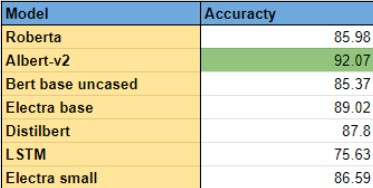
\includegraphics{accuracy.jpg}
\end{center}
\caption[ความแม่นยำในการทำนายของโมเดลแต่ละแบบ]{ความแม่นยำในการทำนายของโมเดลแต่ละแบบ}
\label{fig:ความแม่นยำในการทำนายของโมเดลแต่ละแบบ}
\end{figure}


\section{โปรแกรมอ่านรายงานประจำปีของบริษัท}

\enskip \enskip \enskip เมื่อได้โมเดลที่ดีที่สุดสำหรับการการจำแนกชนิดประโยคซึ่งก็คือ Albert-v2  
เราจึงทดลองนำโมเดลนั้นไปสร้างโปรแกรมสำหรับจำแนกประโยคของรายงานประจำปีทั้งเล่มในทุกๆปีย้อนหลัง5ปีของบริษัทที่ใส่เข้าเป็นอินพุต
โดยเมื่อเราได้ทดลองใช้โปรแกรมนั้นกับหลายๆบริษัทแล้ว จากผลลัพธ์ที่ได้เราจึงได้ข้อมูลที่สรุปได้ว่าบริษัทส่วนมากมักมีแนวโน้มในการพูดถึงประโยคที่เกี่ยวข้องกับสิ่งแวดล้อมและสังคมเพิ่มมากขึ้นทุกปี
ซึ่งอาจเป็นเพราะประเด็นของESGที่กำลังได้รับความนิยมในปัจจุบัน
และประโยคส่วนมากเป็นประโยคที่เกี่ยวข้องกับธรรมาภิบาลและไม่เกี่ยวข้องกับประเด็นไหนเลย
เพราะในรายงานประจำปีมักมีการพูดถึงเรื่องการบริหารจัดการในบริษัทเป็นจำนวนมากและเรื่องอื่นๆที่ไม่เกี่ยวข้องกับประเด็นESGก็มีอยู่มากเช่นกัน

\begin{figure}
\begin{center}
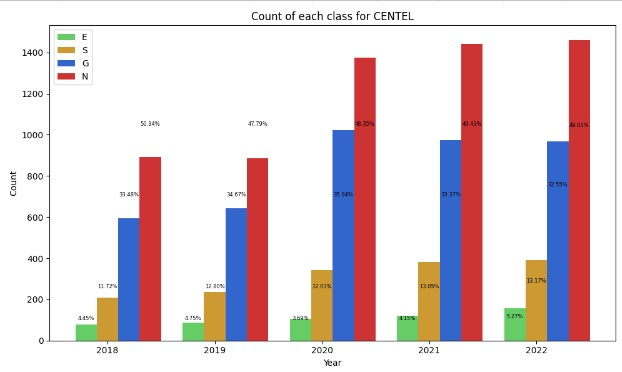
\includegraphics{graph.jpg}
\end{center}
\caption[ทดลองใช่โปรแกรมอ่านรายงานประจำปีของบริษัท CENTEL]{ทดลองใช่โปรแกรมอ่านรายงานประจำปีของบริษัท CENTEL}
\label{fig:ทดลองใช่โปรแกรมอ่านรายงานประจำปีของบริษัท CENTEL}
\end{figure}
\ifproject
\chapter{\ifenglish Conclusions and Discussions\else บทสรุปและข้อเสนอแนะ\fi}

\section{\ifenglish Conclusions\else สรุปผล\fi}

\enskip \enskip \enskip ในการทำโครงงานนี้สามารถพัฒนาระบบที่ใช้ในการจำแนกประเภทประโยคในรายงานประจำปีอัตโนมัติ
โดยระบบนี้มีความแม่นยำถึง 92.07 \% และประโยคที่ทำนายผิดก็มักเป็นประโยคที่จำแนกได้ยากจริงๆแม้จะให้มนุษย์มาจำแนกเองและได้ทำการทดลองนำไปใช้กับรายงานประจำปีทั้งเล่มในหลายๆปีและหลายๆบริษัทแล้วก็ได้พบว่ามีแนวโน้มที่หลายๆบริษัทมักมีเหมือนกันดังที่เห็นในผลลัพธ์จากหัวข้อ4.2



\section{\ifenglish Challenges\else ปัญหาที่พบและแนวทางการแก้ไข\fi}

\enskip \enskip \enskip ในการทำโครงงานนี้ พบว่าเกิดปัญหาหลักๆ ดังนี้


\begin{enumerate} 
    \item
    การหาวิธีในการจำแนกประโยคในรายงานประจำปีของแต่ละบริษัทเพื่อใช้สำหรับพัฒนาโมเดลจำแนกประโยค
    \item
    หาวิธีเลือกดึงประโยคที่สมบูรณ์เหมาะสำหรับในการใช้กับโมเดลจำแนกประโยคโดยอัตโนมัติ
\end{enumerate}

\section{\ifenglish%
Suggestions and further improvements
\else%
ข้อเสนอแนะและแนวทางการพัฒนาต่อ
\fi
}

\enskip \enskip \enskip ข้อเสนอแนะเพื่อพัฒนาโครงงานนี้ต่อไป มีดังนี้


\begin{enumerate} 
    \item
    ทำให้โปรแกรมสามารถรับมือกับการจำแนกประโยคที่มีหลายประเด็นของ ESG ในหนึ่งประโยคได้
    \item
    พัฒนาระบบที่ใช้กับรายงานฉบับภาษาไทยได้
\end{enumerate}

\fi

\bibliography{myReport}

\ifproject
\normalspacing
\appendix
\chapter{The first appendix}

% Text for the first appendix goes here.

% \section{Appendix section}

% Text for a section in the first appendix goes here.

% test ทดสอบฟอนต์ serif ภาษาไทย

% \textsf{test ทดสอบฟอนต์ sans serif ภาษาไทย}

% \verb+test ทดสอบฟอนต์ teletype ภาษาไทย+

% \texttt{test ทดสอบฟอนต์ teletype ภาษาไทย}

% \textbf{ตัวหนา serif ภาษาไทย \textsf{sans serif ภาษาไทย} \texttt{teletype ภาษาไทย}}

% \textit{ตัวเอียง serif ภาษาไทย \textsf{sans serif ภาษาไทย} \texttt{teletype ภาษาไทย}}

% \textbf{\textit{ตัวหนาเอียง serif ภาษาไทย \textsf{sans serif ภาษาไทย} \texttt{teletype ภาษาไทย}}}

% \url{https://www.example.com/test_ทดสอบ_url}

\chapter{\ifenglish Manual\else คู่มือการใช้งานระบบ\fi}

\section{คู่มือการดาวน์โหลดโปรแกรม}

\enskip \enskip \enskip การใช้งานโปรแกรมขั้นแรก 
ผู้สนใจทดลองใช้โปรแกรมสามารถค้นหาและดาวน์โหลดโปรแกรมได้ที่ 
https://github.com/Gravitumn/ESG-classification 


\section{คู่มือการฝึกสอนโมเดลเพิ่มเติม}

\enskip \enskip \enskip ผู้ที่มีความสนใจจะฝึกสอนโมเดลเพิ่มเติมสามารถทำการเรียกใช้ฟังก์ชัน 
Train\_model ซึ่งอยู่ภายในไฟล์ Train.py ได้ โดยมี Arguments ที่สามารถส่งเข้าไปในฟังก์ชันได้ดังนี้


\begin{enumerate} 
    \item
    bert\_model เป็น argument ที่ใช้ในการระบุโมเดลที่ใช้ในการฝึกสอนโดยใช้ file path ในการระบุ หากต้องการใช้โมเดลที่ฝึกสอนโดยผู้จัดทำ สามารถใช้ไฟล์ model/albert2 ซึ่งเตรียมไว้ให้ในโฟลเดอร์ได้เลย
    แต่หากต้องการใช้โมเดลชนิดอื่นก็สามารถใส่ path ดังตัวอย่างด้านล่างได้เช่นกัน
    \item
    tokenizer เป็นการระบุ tokenizer ที่จะใช้ในการแบ่งประโยคซึ่งโดยปกติจะใช้เป็น
    tokenizer ของโมเดลนั้นๆ ดังตัวอย่างด้านล่าง
    \item
    device เป็นการระบุอุปกรณ์ที่ใช้ในการฝึกสอน ตามตัวอย่างด้านล่าง
    \item
    file\_path ของ dataset ที่เราจัดเตรียมไว้ 
    โดยไม่จำเป็นต้องแบ่ง Train/test เนื่องจาก จะมีให้ระบุเป็น Argument 
    \item
    batch\_size เป็นพารามิเตอร์ของการฝึกสอนโมเดลที่ช่วยให้โมเดลเรียนรู้ได้ดีมากขึ้นหากปรับได้อย่างเหมาะสม 
    นอกจากนี้การปรับให้มี batch\_size ที่สูงเกินไปยังส่งผลให้หน่วยความจำของคอมพิวเตอร์ไม่เพียงพออีกด้วย โดยมี default batch size = 8
    \item
    Shuffle เป็นพารามิเตอร์ที่ใช้ระบุว่าต้องการสับเปลี่ยนการเรียงลำดับของ dataset 
    หรือไม่ซึ่งมีค่า default เป็น True และแนะนำให้ตั้งค่าเป็น True เสมอ
    \item
    lr หรือ learning\_rate เป็นพารามิเตอร์ที่ใช้ในการระบุ 
    learning rate ในการเรียนรู้ของคอมพิวเตอร์ มีค่า default = 1e-5
    \item
    num\_epochs เป็นพารามิเตอร์ที่ใช้ในการระบุว่าโมเดลจะได้รับการฝึกสอนเป็นจำนวนกี่ครั้ง 
    โดยมีค่า default = 100
    \item
    T\_0 เป็นพารามิเตอร์สำหรับ Cosine annealing warm restart โดย T\_0 จะเป็นตัวกำหนดว่าจะให้โมเดลทำการเรียนรู้กี่ epoch ก่อนจะเกิดการ restart ซึ่งในระหว่างนั้นจะมีการปรับ learning rate ให้ต่ำลงและเมื่อเกิดการ restart จะทำให้ learning rate 
    กลับมาเท่ากับค่าเริ่มต้น ช่วยให้โมเดลสามารถเรียนรู้ต่อไปได้ มีค่า default= 2
    \item
    T\_mult เป็นพารามิเตอร์สำหรับ Cosine annealing warm restart เป็นตัวคูณซึ่งใช้ในการกำหนดจำนวนรอบก่อนจะเริ่ม restart อีกครั้งหนึ่ง ยกตัวอย่างเช่นหาก T\_mult = 2 และ T\_0 = 10 เมื่อเกิดการ restart จะต้องรออีก 20 ครั้งเพื่อจะ restart และหลังจากนั้นจะเพิ่มเป็น 40 ครั้ง 
    และ 80 ครั้งจนกว่าจะพบเงื่อนไขการจบการฝึกสอน โดยมีค่า default = 2
    \item
    eta\_min เป็นพารามิเตอร์สำหรับกำหนดว่า learning\_rate สามารถลดลงต่ำสุดได้มากเพียงใด 
    เพื่อไม่ให้ learning\_rate ลดต่ำจนเกินไป โดยมีค่า default = 1e-6
    \item
    model\_save\_path เป็น argument สำหรับระบุ file path ที่จะใช้ในการบันทึกโมเดลเมื่อจบการฝึกสอน 
    โดยมี default path เป็น /model/trained\_model
    \item
    early\_stop\_epoch เป็น argument สำหรับระบุจำนวนรอบสูงสุดที่ต้องการให้โมเดลทำการฝึกสอน
    โดยมีค่าตั้งต้น = 8 รอบ
    \item
    return\_result เป็น argument สำหรับระบุว่าผู้ใช้งานต้องการผลลัพธ์จากการฝึกสอนหรือไม่ โดยผลลัพธ์เหล่านี้จะเป็น confusion matrix ที่แสดงการทำนายประโยคของโมเดล 
    และกราฟ accuracy ในแต่ละ epoch โดยมีค่า default = False
    \item
    test\_size เป็น argument สำหรับการทำ train\-test\-split 
    โดยมีค่าเริ่มต้น = 0.1 ซึ่งเป็นการระบุว่าใช้ test set 10\% ของ dataset
    \item
    random\_state เป็น argument สำหรับใช้ระบุว่าจะทำการ train\-test\-split 
    ที่ random\_state เท่าใด โดยมีค่าตั้งต้นเป็น 69
\end{enumerate}





%% Display glossary (optional) -- need glossary option.
\ifglossary\glossarypage\fi

%% Display index (optional) -- need idx option.
\ifindex\indexpage\fi

\begin{biosketch}
\begin{center}
  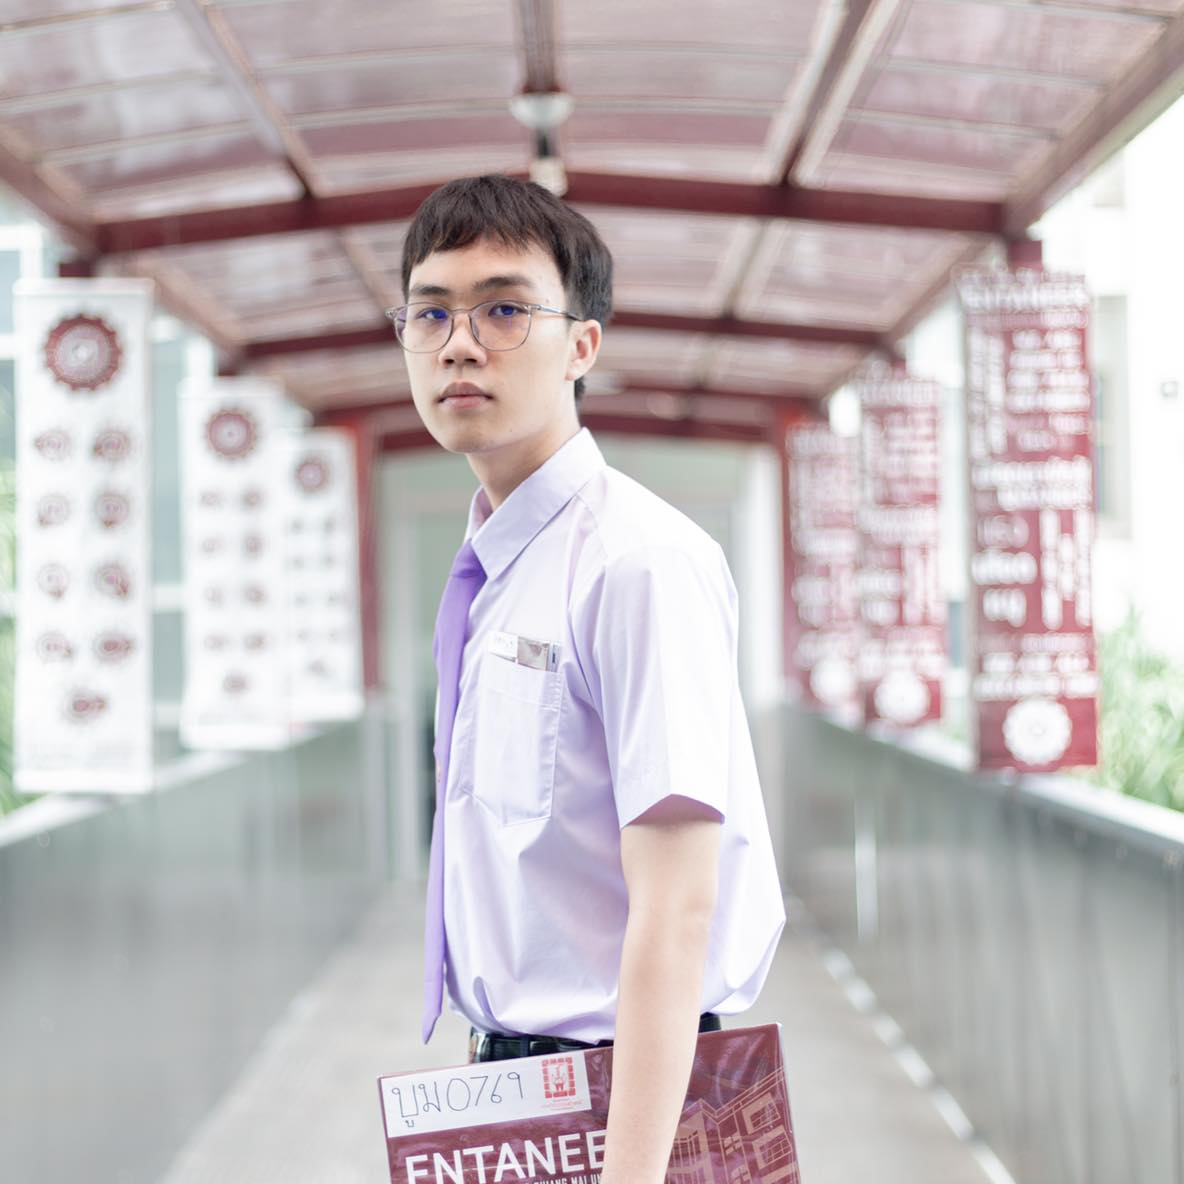
\includegraphics[width=1.5in]{supak.jpg}
\end{center}
นาย สุภาค ไชยเนตรเกษม เกิดเมื่อวันที่ 25 เมษายน 2545 ณ จังหวัดแพร่
สำเร็จการศึกษาระดับมัธยมจากโรงเรียนพะเยาพิทยายม เข้าศึกษาที่ภาควิชาวิศวกรรมคอมพิวเตอร์
มหาวิทยาลัยเชียงใหม่ เมื่อปีการศึกษา 2563 โดยมีความสนใจในด้าน Artificial Intelligence
และ Natural Language Processing

  \begin{center}
    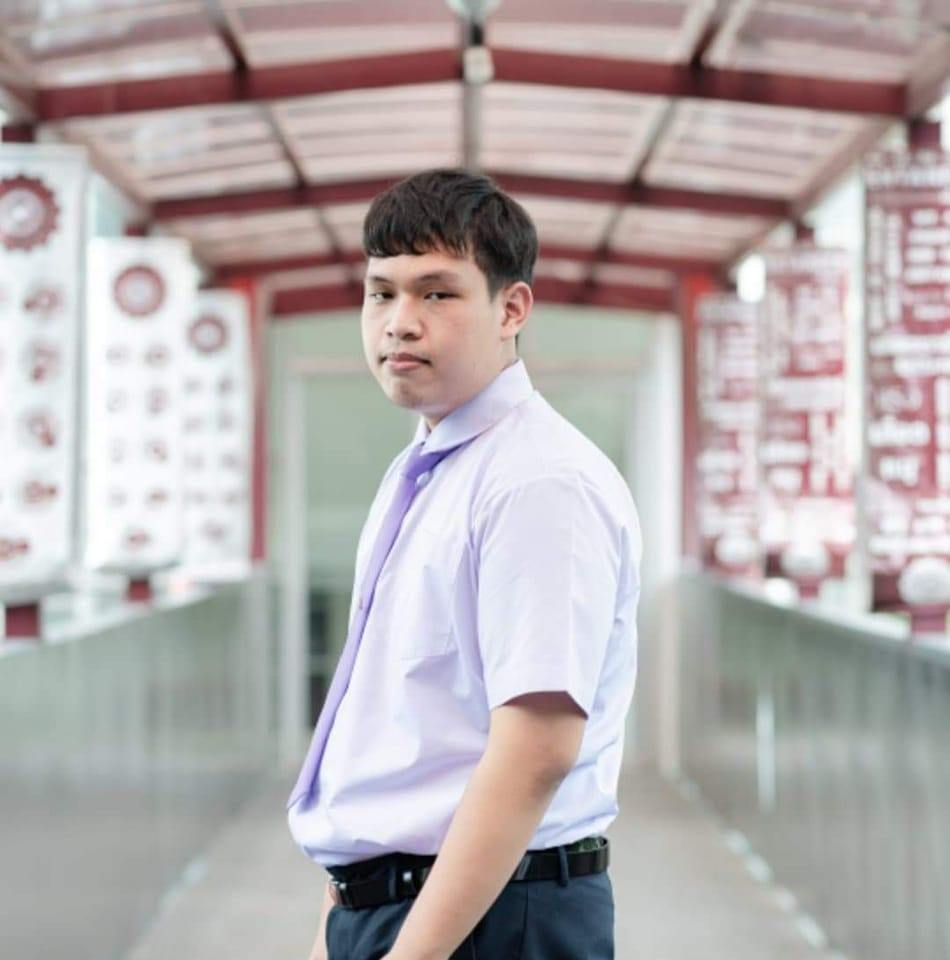
\includegraphics[width=1.5in]{thanisorn.png}
  \end{center}
  นาย ธนิสร ไชยวุฒิ เกิดเมื่อวันที่ 12 กุมภาพันธ์ 2545 ณ จังหวัดพะเยา
  สำเร็จการศึกษาระดับมัธยมจากโรงเรียนพะเยาพิทยายม เข้าศึกษาที่ภาควิชาวิศวกรรมคอมพิวเตอร์
  มหาวิทยาลัยเชียงใหม่ เมื่อปีการศึกษา 2563 โดยมีความสนใจในด้าน Artificial Intelligence
  และ Natural Language Processing
  \end{biosketch}
\fi % \ifproject
\end{document}
